\chapter{Software Requirement Specification}
\section{Use-cases}

The following use cases illustrate the functionality and interactions of the HealthFlow Connect system:

\subsection{Admin Management}

\begin{enumerate}[label=\textbf{UC\arabic*.}]
  \item \textbf{Manage Users:} The admin can create, update, and delete user accounts for doctors, pharmacists, counters, and lab technicians.
  
  \item \textbf{Generate Reports:} The admin can generate reports on user activity, patient data, and system performance for analysis and decision-making.
\end{enumerate}

\subsection{Doctor Interaction}

\begin{enumerate}[label=\textbf{UC\arabic*.}]
  \item \textbf{Diagnose Patient:} The doctor can input patient complaints, conduct general examinations, prescribe medications, and order lab tests for diagnosis.
  
  \item \textbf{Access Patient History:} The doctor can access the entire medical history of a patient, including past diagnoses, treatments, and medications prescribed.
  
  \item \textbf{Update Case Paper:} The doctor updates the patient's case paper with new information during each visit or consultation.
\end{enumerate}

\subsection{Counter Operations}

\begin{enumerate}[label=\textbf{UC\arabic*.}]
  \item \textbf{Create New Patient Record:} The counter staff creates a new patient record, including demographic information and initial symptoms.
  
  \item \textbf{Update Patient Record:} The counter staff updates existing patient records with any changes in personal information or medical history.
  
  \item \textbf{Print Case Paper:} The counter staff prints the patient's case paper for reference during consultations or referrals.
\end{enumerate}

\subsection{Lab Technician Tasks}

\begin{enumerate}[label=\textbf{UC\arabic*.}]
  \item \textbf{View Lab Tests:} The lab technician views the list of lab tests to be performed for a patient.
  
  \item \textbf{Enter Test Results:} The lab technician enters and uploads test results in the form of documents or images.
  
  \item \textbf{Update Patient Records:} The lab technician updates the patient's case paper with the completed lab test results.
\end{enumerate}

\subsection{Pharmacist Functions}

\begin{enumerate}[label=\textbf{UC\arabic*.}]
  \item \textbf{View Medications:} The pharmacist views the list of medications prescribed to a patient.
  
  \item \textbf{Dispense Medications:} The pharmacist dispenses medications to patients and updates their records accordingly.
\end{enumerate}

These use cases demonstrate the various interactions and functionalities of the HealthFlow Connect system, catering to the needs of different user roles and facilitating seamless healthcare management and delivery.

\clearpage % Force a new page to better organize content

\section{Use Case View}
\subsection{Admin Staff UCD}
\begin{figure}[h!]
    \centering
    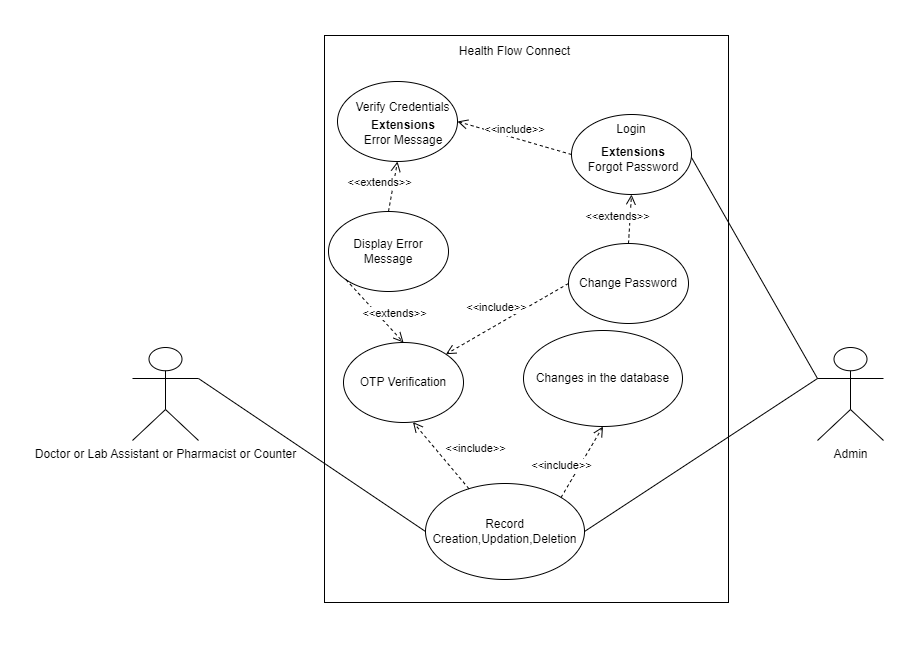
\includegraphics[width=1.1\textwidth]{Admin_Staff_UCD.png}
    \caption{Admin Staff UCD}
    \label{fig:admin_staff_ucd}
\end{figure}
\clearpage
\subsection{Patient Counter UCD}
\begin{figure}[h!]
    \centering
    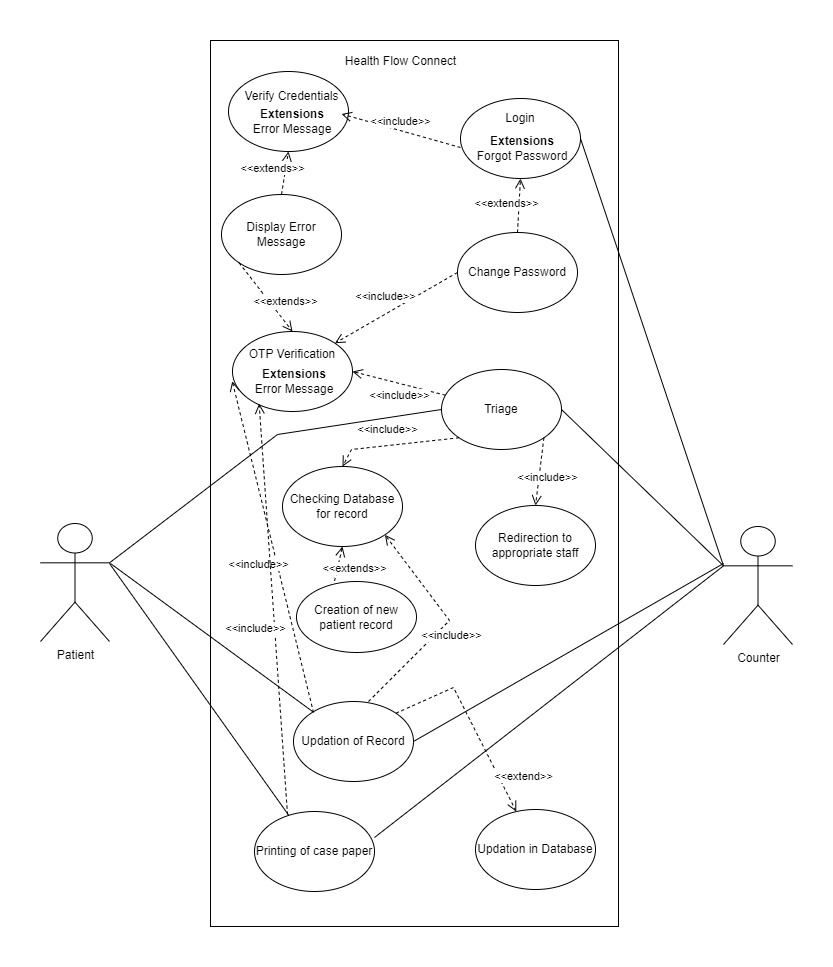
\includegraphics[width=1.1\textwidth]{Patient_Counter_UCD (1).jpg}
    \caption{Patient Counter UCD}
    \label{fig:patient_counter_ucd}
\end{figure}
\clearpage
\subsection{Patient Doctor UCD}
\begin{figure}[h!]
    \centering
    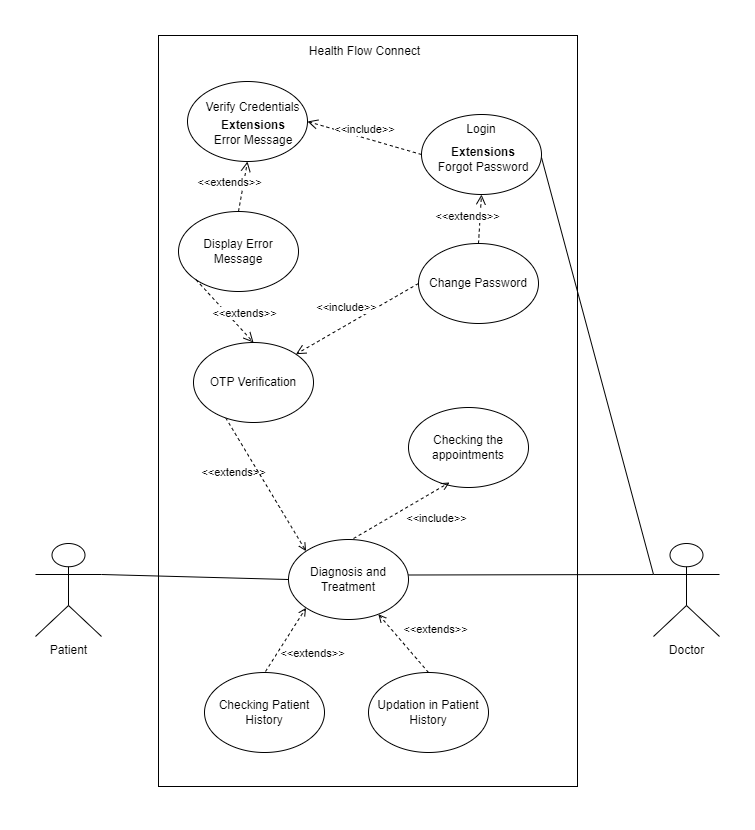
\includegraphics[width=1.1\textwidth]{Patient_Doctor_UCD.png}
    \caption{Patient Doctor UCD}
    \label{fig:patient_doctor_ucd}
\end{figure}
\clearpage
\subsection{Patient Lab Assistant UCD}
\begin{figure}[h!]
    \centering
    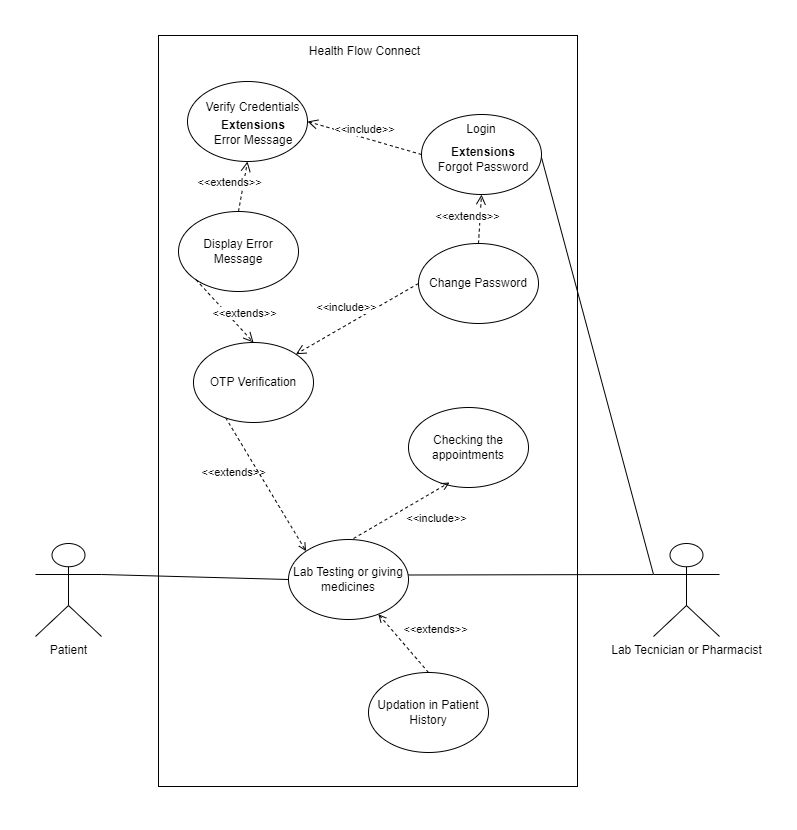
\includegraphics[width=1.1\textwidth]{Patient_Lab_Assistant_Pharmacist_UCD.png}
    \caption{Patient Lab Assistant UCD}
    \label{fig:patient_lab_pharmacist_ucd}
\end{figure}
\clearpage
\section{Data Model and Description} 
\subsection{Data Description}
\begin{table}[h]
\centering
\begin{tabular}{|p{3cm}|p{4cm}|p{6cm}|}
\hline
\textbf{Entity} & \textbf{Attributes} & \textbf{Description} \\
\hline
Users & username, password, designation & Individuals with access to the system \\
Doctors & person ID, OPD, degrees, specializations, admin status & Medical practitioners \\
Patients & UID, name, age, gender, address, contact number, medical history & Individuals receiving medical treatment \\
Case Papers & patient UID, history ID array, start date/time, end date/time, active status & Medical records for patients \\
History Records & patient UID, user UID, user role, date/time, complaints, examination details, lab tests, medications, extra notes & Detailed medical history for patients \\
\hline
\end{tabular}
\end{table}
\begin{table}[h]
\centering
\begin{tabular}{|p{3cm}|p{4cm}|p{6cm}|}
\hline
Lab Technicians & person ID, degrees, specializations, lab type & Staff responsible for laboratory testing \\
Pharmacists & person ID, degrees, specializations & Staff responsible for medication dispensing \\
Redirection Records & patient UID, user UID, user role, redirection creation date/time, redirection served date/time, redirection status, respective history ID, lab testings to be done, medicines to be given & Tracks patient redirections between staff members \\
Persons & UID, first name, middle name, last name, gender, date of birth, phone number, address, role & Individuals involved in the healthcare process \\
\hline
\end{tabular}
\caption{Database Entities}
\end{table}
\clearpage
\subsection{Entity relationship diagram}
\begin{figure}[h!]
    \centering
    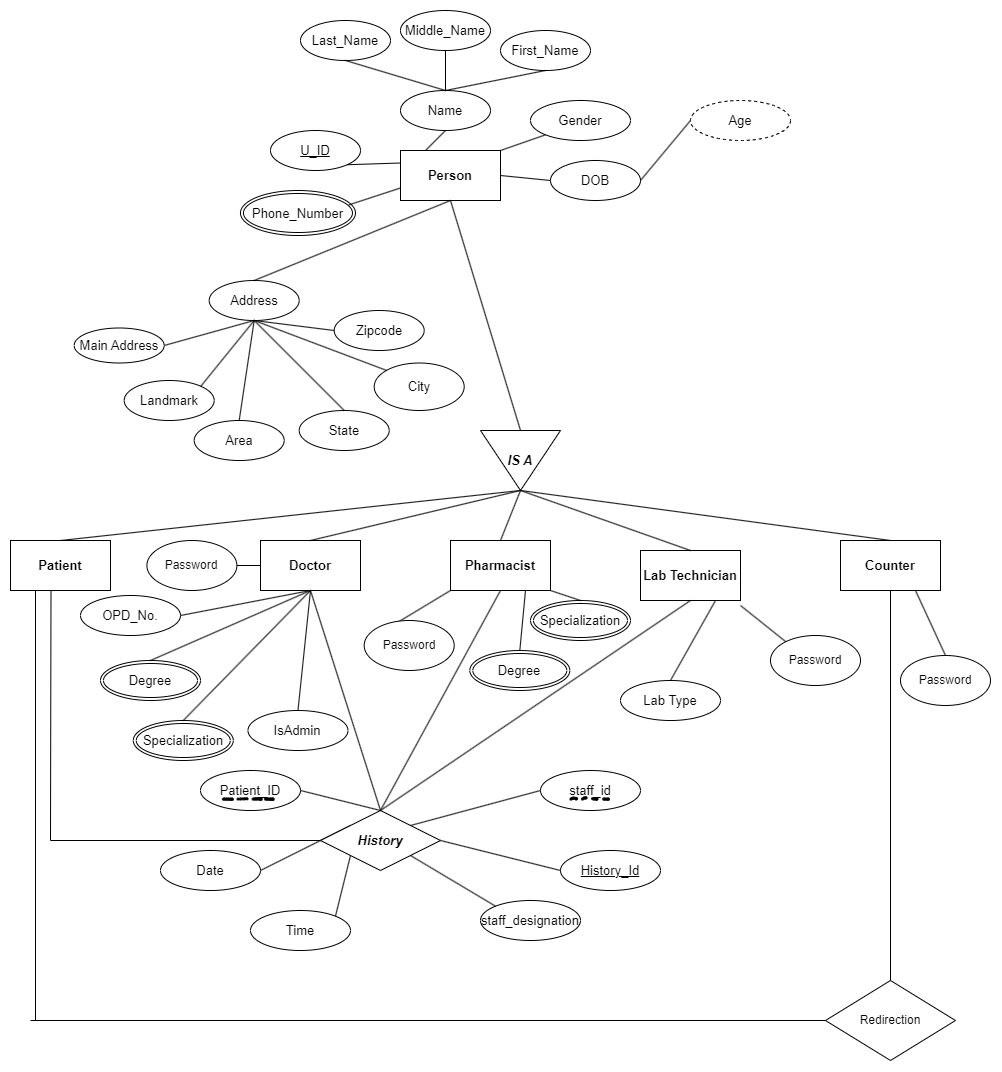
\includegraphics[width=1.1\textwidth]{erd.png}
    \caption{Entity relationship diagram}
\end{figure}
\clearpage

\section{Data Flow Digrams}
\subsection{Level 0 DFD}
\begin{figure}[h!]
    \centering
    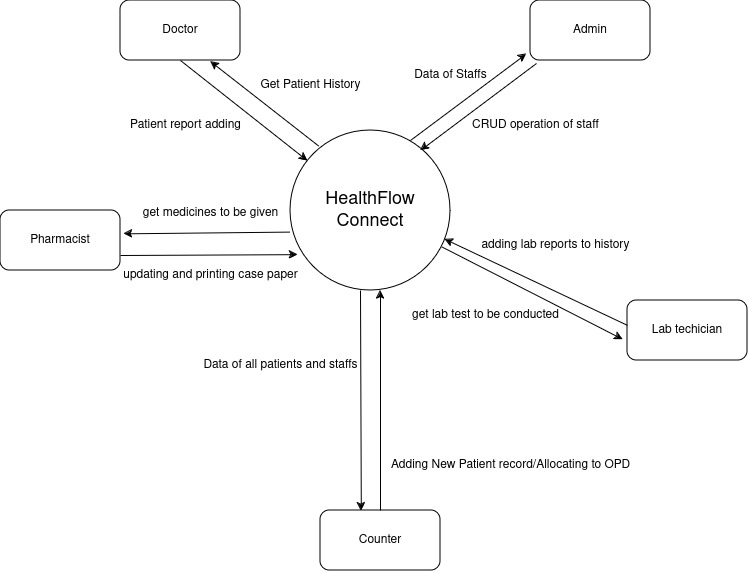
\includegraphics[width=1.1\textwidth]{level0dfd.jpg}
    \caption{Level 0 DFD}
\end{figure}
\clearpage
\subsection{Level 1 DFD}
\begin{figure}[h!]
    \centering
    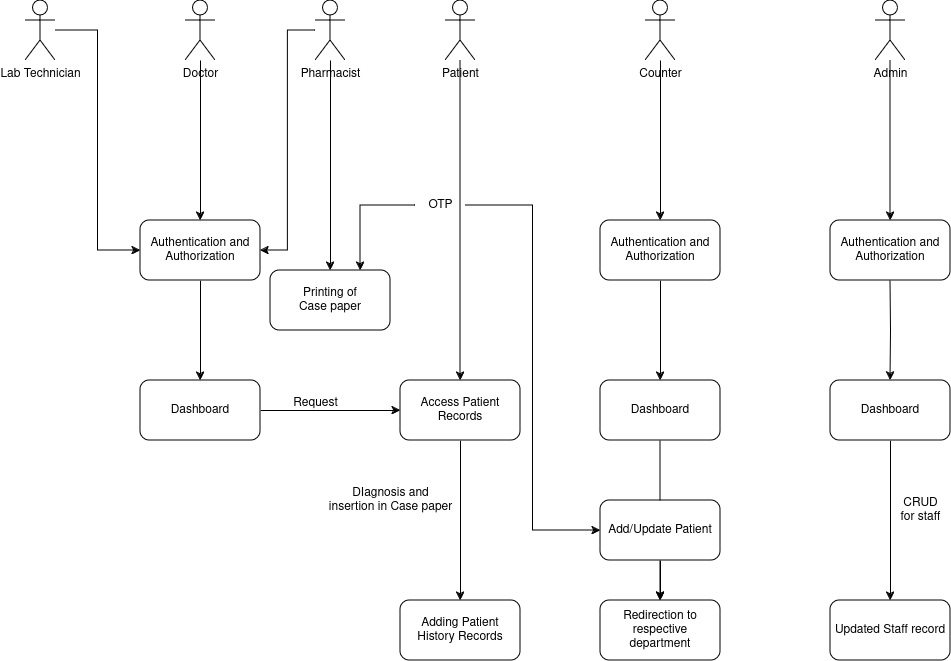
\includegraphics[width=1.1\textwidth]{level1dfd.jpg}
    \caption{Level 1 DFD}
\end{figure}
\clearpage
\subsection{Level 2 DFD}
\begin{figure}[h!]
    \centering
    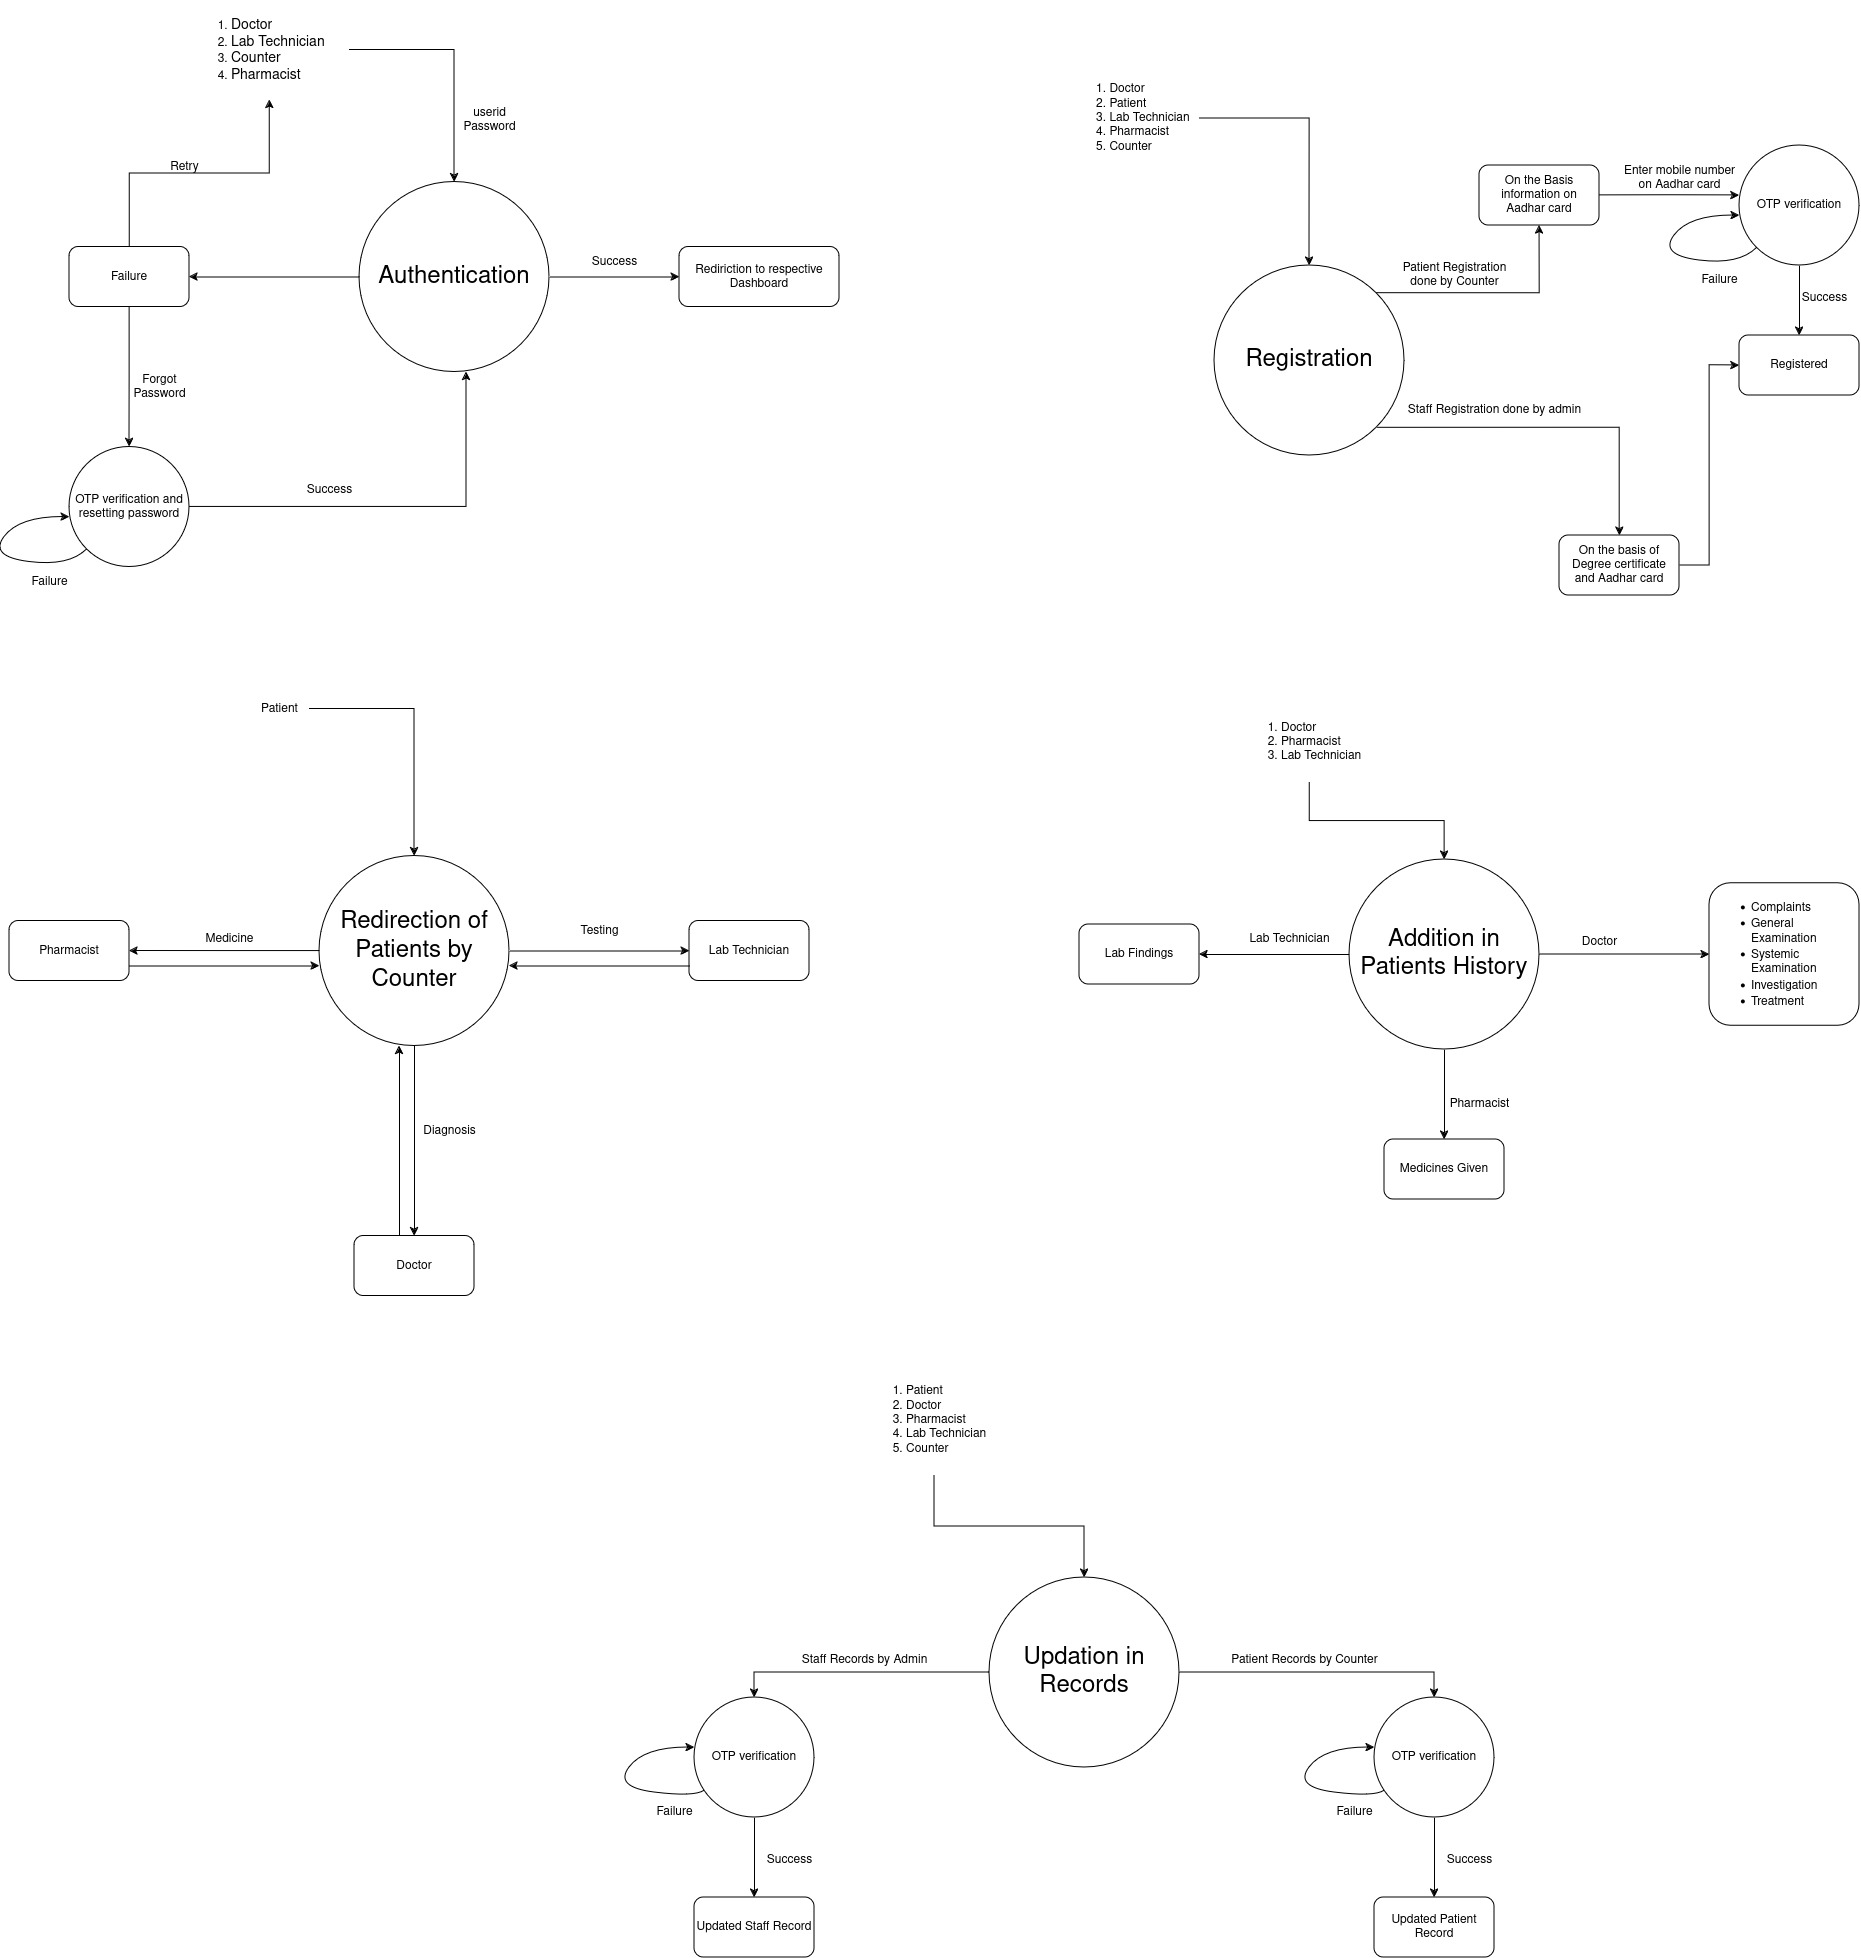
\includegraphics[width=1.1\textwidth]{level2dfd.jpg}
    \caption{Level 2 DFD}
\end{figure}
\clearpage
\section{Description of functions} 
\begin{figure}[h!]
    \centering
    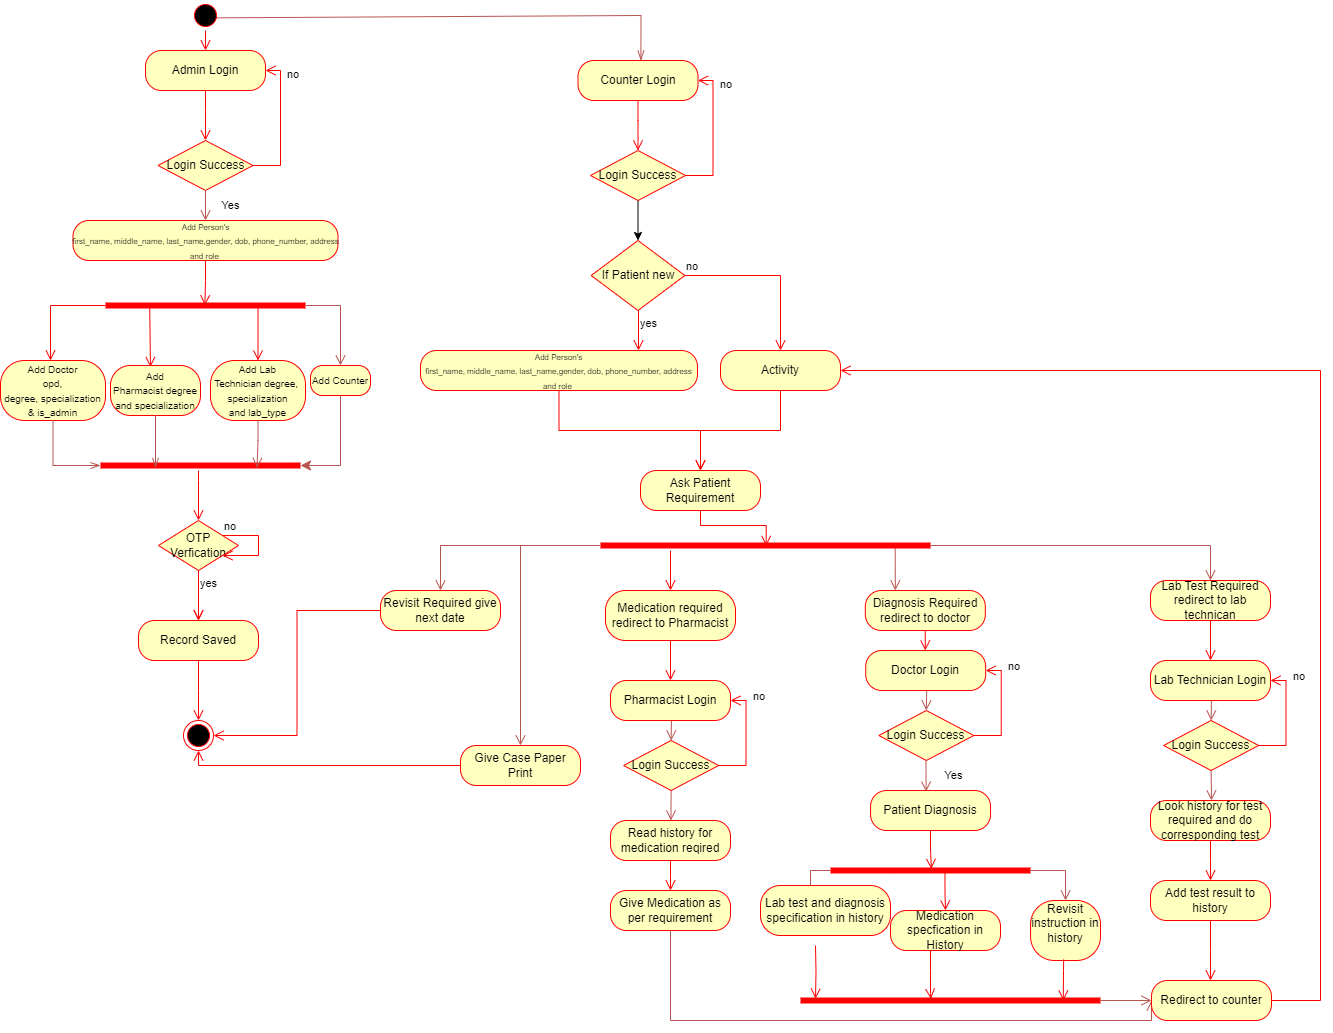
\includegraphics[width=1.1\textwidth]{activity.png}
    \caption{Activity Diagram}
\end{figure}

\subsection{Non Functional Requirements}
\begin{enumerate}[label=\textbf{NF\arabic*.}, leftmargin=*] % Customize labels and indentation
    \item \textbf{Performance}:
    \begin{itemize}[label=--, leftmargin=*] % Customize sub-list appearance
        \item The system should respond to user interactions within a few seconds.
        \item Reports generation should be completed within a few  minutes for datasets of size huge amount of records.
    \end{itemize}
    \clearpage
    \item \textbf{Reliability}:
    \begin{itemize}[label=--, leftmargin=*]
        \item The system should have an uptime of high as possible.
        \item Reports should be accurate and reliable, with less error rate.
    \end{itemize}
    
    \item \textbf{Scalability}:
    \begin{itemize}[label=--, leftmargin=*]
        \item The system should be able to handle a growing user base without significant degradation in performance.
        \item It should support adding additional hardware resources to accommodate increased load.
    \end{itemize}

    \item \textbf{Security}:
    \begin{itemize}[label=--, leftmargin=*]
        \item Access to sensitive information should be restricted based on user roles and permissions.
        \item The system should implement measures to prevent unauthorized access, such as authentication and authorization mechanisms.
    \end{itemize}

    \item \textbf{Maintainability}
    \begin{itemize}[label=--, leftmargin=*]
        \item The codebase should be well-documented and follow coding standards.
        \item It should be easy to modify or extend the system to accommodate future requirements.
    \end{itemize}
\end{enumerate}
\clearpage
